\chapter{Neural Network}

An artificial neural network network mimics the working of a real brain. The brain exists of neurons that transmit information via synapseses. The computer science way to mimic these neurons is shown in figure \ref{fig:nnd}. These work in the bigger context as shown in figure \ref{fig:nno}. In this figure you see different kinds of layers, the input layer (which handles the input), the hidden layer(s) (which pass information) and the output layer (the results). To go from one layer to next you weight the input data, and pass it through the function in the neuron. The function in the neuron is a threshold function (aka activiation function). It is basically the sum of all of the weighted values above or below a certain value. If it is above the threshold the neuron fires a signal (1) otherwise it fires (0). This in turn is then weighted and passed to the next neuron untill the output layer is reached. To optimise we can actually drop the threshhold value (thanks to Paul Werbos) and use a sigmoid function instead for making the decisions. The weights are initially chosen at random and will be optimised later on.
\\\\
In a typical feed forward neural network you first pass the information through the network and then you compare your output layer to the hoped results. From here you begin adjusting the weights to minimise loss/cost, this is called backpropagation. This is an optimisation problem that can be used using for example stochastic gradient descent (or more recent options like AdaGrad and the Adam Optimiser). Once all your examples (and you need a lot of examples) are run and your network is optimised, you can start using this network to make often very good predictions.
\\\\
Sometimes dropouts are used to mimic dead neurons in the brain. This decreases the chance of over-weighted, or otherwise biasing, neurons in the artificial neural network.

\section{Feed Forward Neural Networks}
A feed forward neural network simply passes the information straight through the neural net and uses backpropagation to optimise the weights. For a sentiment predictor Neural Net implementation look at appendix \ref{code:sentiment} and for an example implementation for number recognition take a look at appendix \ref{code:number-recognition}.

\subsection{Code}
A simple code example of a Feed Forward Neural Network using TensorFlow can be found in appendix \ref{code:nn-example}. 

\section{Recurrent Neural Networks}
Addresses the necessity of understanding data in sequences. In RNN the output of the previous cyclus is used in the activiation function of this cyclus.

\subsection{LSTM}
The Long Short Term Memory cell determines the weight of the previous output and the current input so that your initial input doesn't start to dominate the output. Basically it decides what data to keep and what data to forget.
See link\footnote{http://colah.github.io/posts/2015-08-Understanding-LSTMs/} for more information.

\subsection{Code}
A simple code example of a LTSM using TensorFlow can be found in appendix \ref{code:ltsm}. 

\section{Convolutional Neural Network}
Convolution takes the original data and creates feature maps from it. Pooling is the same as down-sampling. Most often used is max-pooling where a region is selected and all values of the region is set equal to the maximum value in that region. The fully connected layer is your typical multilayer perceptron. It roughly has the following structure:
\begin{enumerate}
\item Convolution
\item Pooling
\item Convolution
\item Pooling
\item Fully Connected Layer
\item Output
\end{enumerate}

\begin{figure}
\centering
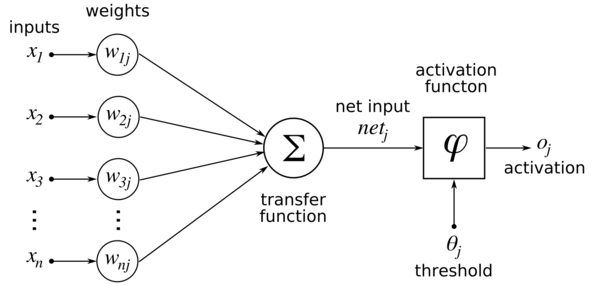
\includegraphics[width=0.8\textwidth]{images/nn_detail.png}
\caption{\label{fig:nnd} Shows the detailed working for one node in an artificial neural network.}
\end{figure}

\begin{figure}
\centering
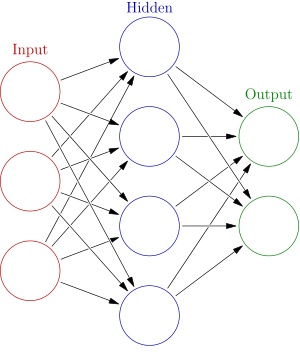
\includegraphics[width=0.4\textwidth]{images/nn_overview.png}
\caption{\label{fig:nno} Shows the general overview of an artificial neural network.}
\end{figure}

\subsection{Code}
A simple code example of a Convolutional Neural Network using TensorFlow can be found in appendix \ref{code:cnn}. For an implementation of the same code using TFLearn take a look at appendix \ref{code:tflearn}